\documentclass[tikz,border=3pt]{standalone}
\usepackage[utf8]{inputenc}
\usepackage[T1]{fontenc}
\usepackage{lmodern}
\renewcommand{\familydefault}{\sfdefault}
\usepackage{sansmath}\sansmath
\usepackage{chemfig}
\usepackage{pgfplots}\pgfplotsset{compat=1.18,/pgf/number format/use comma,/pgf/number format/1000 sep={.}}
\usetikzlibrary{arrows.meta,calc,positioning,decorations.pathmorphing,patterns}
% paleta del sitio
\definecolor{nar}{HTML}{E8680C}\definecolor{narc}{HTML}{FFB35C}\definecolor{hielo}{HTML}{FFF3E8}
\definecolor{tinta}{HTML}{1D1D1F}\definecolor{gris}{HTML}{6E6E73}\definecolor{lila}{HTML}{7C5CF0}
\definecolor{azul}{HTML}{2F6FD6}\definecolor{menta}{HTML}{17A673}\definecolor{coral}{HTML}{E8342A}
\begin{document}
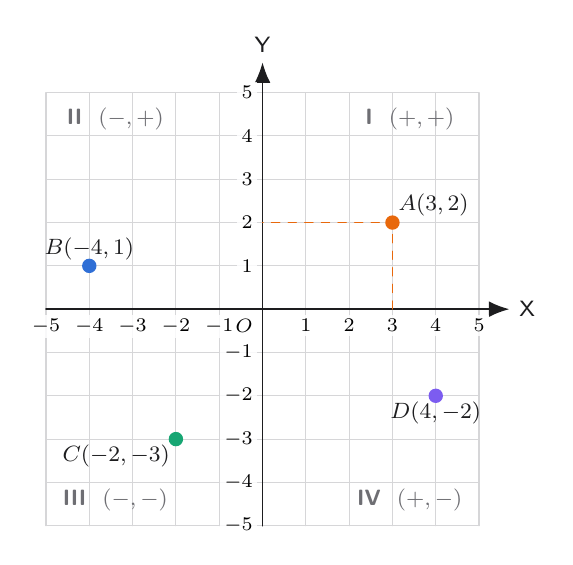
\begin{tikzpicture}[font=\small,x=0.55cm,y=0.55cm,line cap=round,line join=round,step={(1,1)}]
\draw[gris!28,thin] (-5,-5) grid (5,5);
\draw[-{Latex[length=2.6mm,width=2mm]},tinta,semithick] (-5,0)--(5.7,0) node[right,font=\footnotesize] {X};
\draw[-{Latex[length=2.6mm,width=2mm]},tinta,semithick] (0,-5)--(0,5.7) node[above,font=\footnotesize] {Y};
\node[below,font=\scriptsize,inner sep=1.5pt,fill=white,fill opacity=.85,text opacity=1] at (-5,-0.12) {$-5$};
\node[below,font=\scriptsize,inner sep=1.5pt,fill=white,fill opacity=.85,text opacity=1] at (-4,-0.12) {$-4$};
\node[below,font=\scriptsize,inner sep=1.5pt,fill=white,fill opacity=.85,text opacity=1] at (-3,-0.12) {$-3$};
\node[below,font=\scriptsize,inner sep=1.5pt,fill=white,fill opacity=.85,text opacity=1] at (-2,-0.12) {$-2$};
\node[below,font=\scriptsize,inner sep=1.5pt,fill=white,fill opacity=.85,text opacity=1] at (-1,-0.12) {$-1$};
\node[below,font=\scriptsize,inner sep=1.5pt,fill=white,fill opacity=.85,text opacity=1] at (1,-0.12) {$1$};
\node[below,font=\scriptsize,inner sep=1.5pt,fill=white,fill opacity=.85,text opacity=1] at (2,-0.12) {$2$};
\node[below,font=\scriptsize,inner sep=1.5pt,fill=white,fill opacity=.85,text opacity=1] at (3,-0.12) {$3$};
\node[below,font=\scriptsize,inner sep=1.5pt,fill=white,fill opacity=.85,text opacity=1] at (4,-0.12) {$4$};
\node[below,font=\scriptsize,inner sep=1.5pt,fill=white,fill opacity=.85,text opacity=1] at (5,-0.12) {$5$};
\node[left,font=\scriptsize,inner sep=1.5pt,fill=white,fill opacity=.85,text opacity=1] at (-0.12,-5) {$-5$};
\node[left,font=\scriptsize,inner sep=1.5pt,fill=white,fill opacity=.85,text opacity=1] at (-0.12,-4) {$-4$};
\node[left,font=\scriptsize,inner sep=1.5pt,fill=white,fill opacity=.85,text opacity=1] at (-0.12,-3) {$-3$};
\node[left,font=\scriptsize,inner sep=1.5pt,fill=white,fill opacity=.85,text opacity=1] at (-0.12,-2) {$-2$};
\node[left,font=\scriptsize,inner sep=1.5pt,fill=white,fill opacity=.85,text opacity=1] at (-0.12,-1) {$-1$};
\node[left,font=\scriptsize,inner sep=1.5pt,fill=white,fill opacity=.85,text opacity=1] at (-0.12,1) {$1$};
\node[left,font=\scriptsize,inner sep=1.5pt,fill=white,fill opacity=.85,text opacity=1] at (-0.12,2) {$2$};
\node[left,font=\scriptsize,inner sep=1.5pt,fill=white,fill opacity=.85,text opacity=1] at (-0.12,3) {$3$};
\node[left,font=\scriptsize,inner sep=1.5pt,fill=white,fill opacity=.85,text opacity=1] at (-0.12,4) {$4$};
\node[left,font=\scriptsize,inner sep=1.5pt,fill=white,fill opacity=.85,text opacity=1] at (-0.12,5) {$5$};
\node[font=\footnotesize\bfseries,text=gris] at (3.4,4.4) {I \ $(+,+)$};
\node[font=\footnotesize\bfseries,text=gris] at (-3.4,4.4) {II \ $(-,+)$};
\node[font=\footnotesize\bfseries,text=gris] at (-3.4,-4.4) {III \ $(-,-)$};
\node[font=\footnotesize\bfseries,text=gris] at (3.4,-4.4) {IV \ $(+,-)$};
\draw[dashed,nar] (3,0)--(3,2)--(0,2);
\fill[nar] (3,2) circle (2.6pt) node[above right,font=\footnotesize,text=tinta,inner sep=2pt] {$A(3, 2)$};
\fill[azul] (-4,1) circle (2.6pt) node[above,font=\footnotesize,text=tinta,inner sep=2pt] {$B(-4, 1)$};
\fill[menta] (-2,-3) circle (2.6pt) node[below left,font=\footnotesize,text=tinta,inner sep=2pt] {$C(-2, -3)$};
\fill[lila] (4,-2) circle (2.6pt) node[below,font=\footnotesize,text=tinta,inner sep=2pt] {$D(4, -2)$};
\node[below left,font=\scriptsize] at (0,0) {$O$};
\end{tikzpicture}
\end{document}
